\subsection{Shape}

In the final delivery stage, the robot evolved from a technical prototype into a \textbf{fully integrated, character-driven system}. The movement module (previously shaped into a cloud-like base) was transformed into the foundation for a visually expressive and narratively rich design.

\begin{figure}[H]
    \centering
    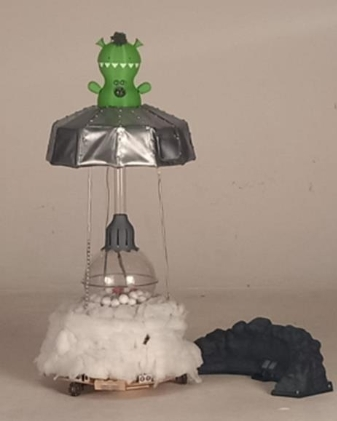
\includegraphics[width=0.6\linewidth]{../ReportMovementModule/images/Aspose.Words.728084da-df58-4b9d-a372-f65cffbdb23d.029.jpeg}
    \caption{Final Robot Design}
\end{figure}

The bottom of the robot remained covered in \textbf{soft white cotton}, representing a storm cloud. This not only gave the robot a magical and playful appearance, but also \textbf{concealed the mechanical components} such as wheels, motors, and sensors. Embedded \textbf{LEDs inside the cotton layer} enhanced the illusion by simulating internal lightning effects, adding a sense of animation and depth.

Rising from this cloud base, a \textbf{transparent vertical column filled with white balls} was installed to symbolize the microwave ticketing mechanism. This interactive visual metaphor helped communicate the robot's core function in a light-hearted way. The structure was topped with a \textbf{dome shaped like a UFO}, reinforcing the fictional theme of an alien-operated machine that has landed in a university setting to distribute turn tickets.

At the peak, a \textbf{green alien figure} served as the face of the robot, further amplifying its friendly and approachable character. This figure helped attract attention and invited interaction, especially in the social environment of a shared student space.

The integration between the modules was carefully planned, both structurally and visually. The cloud base, the transparent ticket chamber, and the dome were aligned with the underlying mechanical layout, while also building a \textbf{consistent narrative language}. Every part contributed to the overall identity of the robot—not just as a machine, but as a \textbf{social object} with personality and purpose.

For full reference, \textbf{all technical drawings and 3D models used in the construction are available via the project repository}. These materials illustrate how the shape was designed, tested, and assembled, and serve as a foundation for future iterations or replication.
